\section{Control} 
\label{sec:control}

% In Section~\ref{sec:em_field} we computed the electric and magnetic fields.
% These fields are depicted in Figure~\ref{fig:wire_w_fields} around the wire
% whose axis is into the page, where the axial component of the electric field is
% ignored since it is many orders of magnitude smaller than its radial component.
% 
% The Poynting vector~\cite{griffiths2014introduction} is given by \[ \bm{P}(s,t)
% = \nicefrac{1}{\mu_0}\bm{E} \times \bm{B}, \] and points axially along the wire.
% Hence, at each point in space around the wire, we can attach a coordinate
% system, $\bm{\Sigma}_w$ whose axes comprises the unit vectors along $\bm{E}$,
% $\bm{P}$, and $\bm{B}$. Since these fields are measured by equipment mounted on
% Astria, they give rise to a rotation matrix between the (extended) wire frame
% and the body frame $\bm{\Sigma}_b$.
% %
% \begin{equation}
%     {^b}R_w = \bmat{\hat{\bm{E}} & \hat{\bm{P}} & \hat{\bm{B}}}.
%     \label{eq:wire_frame}
% \end{equation}
% 
% For manipulation, we want to control Astria's orientation so that its body
% $\bm{y}$-axis aligns with the Poynting vector $\bm{P}$ and move Astria's center
% of mass so that its body $\bm{x}$- and $\bm{z}$-axes align with the electric
% \electric and the magnetic \magnetic fields, respectively.

% We discuss two separate control strategies that utilize the electric field
% measurements in closing the control loop. The first one directly uses the rms
% measurements without trying to estimate the full state, while the second one
% relies on full state estimation prior to forming the control law.

We devise a control strategy that utilizes the rms electric or magnetic field
measurements to guide a drone towards one of the wires for sensor placement.
%
% \subsection{Control through RMS Measurements}
% \label{ssec:ctrl_thru_rms}
%
The square rms values of the electric fields in the transverse plane on a test
point (sensor location) $q = (x, z)$ is given by 
%
\begin{align}
    \begin{split}
        \bar{E}_{x}^2(q) &=
        \frac{1}{2}\sum_{\alpha=1}^3\left(e_{\alpha}^2c_\alpha^2 -
            \sum_{\alpha^\prime > \alpha}^3e_{\alpha}
    e_{\alpha^\prime} c_\alpha c_{\alpha^\prime} \right), \\
        \bar{E}_{z}^2(q) &= \frac{1}{2}\sum_{\alpha=1}^3\left(e_{\alpha
            }^2 s_\alpha^2 - \sum_{\alpha^\prime > \alpha}^3e_{\alpha}
    e_{\alpha^\prime} s_\alpha s_{\alpha^\prime}\right),
    \end{split}
    \label{eq:rms_xz}
\end{align}
%
The sum of these quantities provides a closed-form expression for the square rms
magnitude of the electric field
%
\begin{equation}
    \bar{E}^2 = \frac{1}{2}\sum_{\alpha=1}^3\left(e_\alpha^2 -
    \sum_{\alpha^\prime > \alpha}^3 e_\alpha
    e_{\alpha^\prime} c_{\alpha \alpha^\prime}\right)
    \label{eq:rms}
\end{equation}
%
where $c_{\alpha \alpha^\prime} := \cos{(\theta_\alpha -
\theta_{\alpha^\prime})}$. Using chain rule with the various derivatives derived
in Section~\ref{ssec:derivatives}, we obtain its gradient.
%
% \begin{align}
%     \begin{split}
%         \pd{\bar{E}^2}{x} &= -\frac{1}{\xi} \sum_{\alpha=1}^3 \left(e_\alpha^3
%         \cos{\theta_\alpha} - \frac{1}{2} \sum_{\alpha^\prime \neq 
%     \alpha}^3 e_\alpha e_{\alpha^\prime}^2 \cos{(\theta_\alpha -
%     2\theta_{\alpha^\prime})} \right), \\
%         \pd{\bar{E}^2}{z} &= \frac{1}{\xi} \sum_{\alpha=1}^3 \left(e_\alpha^3
%         \sin{\theta_\alpha} + \frac{1}{2} \sum_{\alpha^\prime \neq 
%     \alpha}^3 e_\alpha e_{\alpha^\prime}^2 \sin{(\theta_\alpha -
%     2\theta_{\alpha^\prime})} \right), \\
%     \end{split}
%     \label{eq:rms_grad}
% \end{align}
\renewcommand*{\arraystretch}{1.25}
%
\begin{align}
    \begin{split}
    &\nabla_q\bar{E}^2 = 2\bar{E}\nabla_q\bar{E} =  
    \frac{1}{2\xi}\sum_{\alpha=1}^3 e_\alpha \times \\
    &\phantom{1234}\bmat{
        -c_\alpha \left( \sum_{\alpha^\prime \neq \alpha} e_\alpha^2 - 2s_\alpha s_{\alpha^\prime}e_\alpha
        e_{\alpha^\prime} + \left(2s_{\alpha^\prime}^2-1\right)e_{\alpha^\prime}^2 \right) \\
        s_\alpha \left( \sum_{\alpha^\prime \neq \alpha} e_\alpha^2 - 2c_\alpha c_{\alpha^\prime}e_\alpha
        e_{\alpha^\prime} + \left(2c_{\alpha^\prime}^2-1\right)e_{\alpha^\prime}^2 \right) \\
    } \\
    &= \frac{1}{2\xi} \sum_{\alpha=1}^3 e_\alpha
    \bmat{
        -2e_\alpha^2 c_\alpha + \sum_{\alpha^\prime \neq \alpha}
        e_{\alpha^\prime}^2
        \cos{\left(\theta_\alpha-2\theta_{\alpha^\prime}\right)}\\
        2e_\alpha^2 s_\alpha + \sum_{\alpha^\prime \neq \alpha} 
        e_{\alpha^\prime}^2
        \sin{\left(\theta_\alpha-2\theta_{\alpha^\prime}\right)}
    }
    \end{split}
    \label{eq:rms_grad}
\end{align}
%
After a fair amount of trigonometric manipulation, one can show that the
gradient is a positive linear combination of vectors $f_\alpha := \left[
\begin{smallmatrix} -c_\alpha & s_\alpha \end{smallmatrix} \right]^\top$ for
$\alpha = 1, 2, 3$. Indeed, the expressions in~\eqref{eq:rms_grad} may
equivalently be written as
%
\begin{align}
    \begin{split}
    \nabla_q\bar{E} &= \frac{1}{4\xi \bar{E}} \sum_{\alpha=1}^3 \sigma_\alpha \bmat{-c_\alpha \\
    s_\alpha}, \\
    \sigma_\alpha &= e_\alpha \left( \sum_{\alpha^\prime=1}^3 e_\alpha^2
    - 2c_{\alpha \alpha^\prime} e_\alpha e_{\alpha^\prime} + e_{\alpha^\prime}^2
    \right).
    \end{split}
    \label{eq:rms_grad_positive}
\end{align}
%
The vector $f_\alpha = \left[ \begin{smallmatrix} -c_\alpha & s_\alpha
\end{smallmatrix} \right]^\top$ can be identified as the unit vector pointing
from the location of a sensor to the $\alpha^{\text{th}}$ transmission wire.
Furthermore, we can readily see that $\sigma_\alpha \geq 0$ for all $\alpha = 1,
2, 3$. Indeed, $e_\alpha > 0$ and
%
\begin{align*} 
    e_\alpha^2 - 2c_{\alpha \alpha^\prime}e_\alpha e_{\alpha^\prime}
    + e_{\alpha^\prime}^2 &= \bmat{e_\alpha & e_{\alpha^\prime}} Q \bmat{e_\alpha
                                           \\ e_{\alpha^\prime}} \geq 0, \\
    Q &= \bmat{
        1 & -c_{\alpha \alpha^\prime} \\ -c_{\alpha \alpha^\prime} & 1
    } \succeq 0.
\end{align*}
%
Here $\succeq$ denotes that the matrix is positive semidefinite, which can be
deduced by computing its principal minors. Therefore, we see that $\sigma_\alpha
\geq 0$ for all $\alpha$. This implies that for
each $q \in \mathbb{R}^2$, the gradient $\nabla_q\bar{E}(q)$ points into the
convex hull (triangle) of the transmission wires, which is our next result. 
\begin{prop}
    Let $\left\{f_i\right\}_{i=1}^3$ denote the unit vectors in $\mathbb{R}^2$
    that point from a given location $q \in \mathbb{R}^2$ to each vertex
    $\left\{v_i\right\}_{i=1}^3$ of a triangle $\mc{T}$. If a vector $v \in
    \mathbb{R}^2$ is a nonnegative linear combination \[ v = \sum_{i=1}^3
    \sigma_i f_i, \quad \sigma_i \geq 0 \] of $\left\{ f_i \right\}_{i=1}^3$
    then the ray it induces $\mc{R} \triangleq \left\{q + sv: s \geq 0\right\}$
    intersects the triangle $\mc{T}$.
\end{prop}

\begin{proof}
    It is well-known that a point in the triangle is a convex combination of its
    vertices. Therefore, the ray $\mc{R}$ intersects the triangle $\mc{T}$ if
    and only if the equation \[ q + sv = (1 - \beta - \gamma)v_1 + \beta v_2 +
    \gamma v_3 \] has a solution such that $\beta, \gamma, s \geq 0$ and $\beta 
    + \gamma \leq 1$. Rearranging the equation and solving it for $v$ yields 
    \[ v = \frac{1}{s}(v_1 - q) + \frac{\beta}{s}(v_2-v_1) +
    \frac{\gamma}{s}(v_3-v_1). \] Notice that $v_i - q = \delta_i f_i$ with
    $\delta_i \geq 0$ for each $i = 1, 2, 3$. Therefore, this last equation may
    be rewritten as \[ v = \frac{\delta_1}{s}(1-\beta-\gamma)f_1 +
    \frac{\delta_2}{s}\beta f_2 + \frac{\delta_3}{s}\gamma f_3 \triangleq
    \sum_{i=1}^3 \sigma_i f_i. \] Notice that $\sigma_i \geq 0$ for each $i = 1,
    2, 3$ due to the constraints on $\beta$, $\gamma$ and $s$, which was to be
    demonstrated.
\end{proof}

\begin{rem}
If the triangle $\mc{T}$ is nondegenerate, there exists $\alpha \in \{1, 2, 3\}$
such that $\sigma_\alpha > 0$. This follows from the above computation of the
matrix $Q$, which is positive definite unless $\theta_\alpha =
\theta_{\alpha^\prime}$, with $\alpha \neq \alpha^\prime$. If the triangle
$\mc{T}$ does not degenerate into a line segment, not all
$\{\theta_\alpha\}_{\alpha=1}^3$ can be equal, implying that there exist an
$\alpha$ such that $\sigma_\alpha > 0$. 
\end{rem}

\begin{rem} \label{rem:extrema}
    The fact that the $\nabla_q\bar{E}$ points into the the triangle $\mc{T}$
    formed by the transmission wires implies, in particular, that the extrema of
    $\bar{E}$ lies in the (closed) triangle.

    Furthermore, since this is an absolute direction, the unit vector along the
    $\nabla_q \bar{E}$ may be used as a bearing factor with respect to which
    localization may be performed. A measure of the ``distance'' to the power
    lines is provided by $\nicefrac{\xi}{\bar{E}}$.
\end{rem}

\subsection{Potential function}
%
We can promote $\bar{E}$ to a compelling potential function $V: \mathbb{R}^2
\rightarrow \mathbb{R}_+$ by choosing
%
\begin{equation}
    V(q) = \dfrac{1}{\bar{E}^2}.
    \label{eq:potential}
\end{equation}
%
This is a nonnegative, decreasing function of $\bar{E}$, with a global minimum
value of zero at $r_\alpha = 0$ for each $\alpha = 1, 2, 3$. Taking the its
gradient, we see that 
%
\begin{equation}
    \nabla_q V(q) = -\dfrac{2}{\bar{E}^3}\nabla_q\bar{E} (q)
    = \frac{1}{4\xi\bar{E}^4} \sum_{\alpha=1}^3 \sigma_\alpha f_\alpha.
    \label{eq:gradV}
\end{equation}
%
Since each $\sigma_\alpha$ is a third-order polynomial of peak electric field
strengths $e_\alpha$, we observe that the magnitude of the gradient
$\nabla_qV(q)$ is of the order $\nicefrac{1}{\bar{E}}$.

\subsection{Behavior of the critical points of the potential function}
\label{ssec:behavior}
%
The negative gradient $-\nabla_qV$ of $V$ points into the triangle $\mc{T}$,
therefore by Remark~\ref{rem:extrema}, we know that it may only vanish
within $\mc{T}$. Equations~(\ref{eq:gradV}, \ref{eq:rms_grad_positive}) combine
to show that the gradient of $V(q)$ vanishes as $e_\alpha \rightarrow \infty$ or
$r_\alpha \rightarrow 0$. 

For an arbitrary three-phase power line configuration, there are two independent
vector loop equations to be satisfied: 
%
\begin{align}
    \begin{split}
        q-v_\alpha + v_{\alpha+1} - q &= v_{\alpha+1} - v_\alpha,  \\
        \frac{\xi}{e_\alpha} \bmat{c_\alpha \\ -s_\alpha} -
        \frac{\xi}{e_{\alpha+1}}\bmat{c_{\alpha+1} \\ -s_{\alpha+1}} &=
        \bmat{x_{\alpha+1} - x_\alpha \\ z_{\alpha+1} - z_\alpha}, \quad \alpha
        = 1, 2.
\end{split}
\label{eq:loopeqn}
\end{align}
%
Simultaneously solving $\nabla_qV(q) = 0$ with the loop
equations~\eqref{eq:loopeqn} provides us with the critical points of the
potential function $V$. Let us coin the term \textit{generic} for a triangle
that is sufficiently far away from being equilateral. It turns out that unless
$\mc{T}$ is ``almost'' equilateral, i.e., generic, then there are $5$ critical
points. $3$ of these $5$ occur at the location of the power lines (vertices of
the triangle $\mc{T}$) and are global minima with a zero value. The remaining
critical points have to be saddle points of $V$, which is our next result.

\begin{lem}
    Let the triangle $\mc{T}$ be generic and $V$ a Morse function. Then the
    remaining two critical points of the potential function $V$ are saddle
    points.
\end{lem}
\begin{proof}
    The Euler characteristic of a triangle is \[ \chi(\mc{T}) = V - E + F = 3 -
    3 + 1 = 1. \] By Poincar\'{e}-Hopf theorem~\cite{burns2005differential}, we
    know that the sum of the indices of the gradient vector field of $V$ equals
    this integer. Since the global minima of $V$ are sinks, they have indices of
    $+1$. This implies that the index of the remaining two critical points must
    sum to $-2$. As long as these two critical points are not located at the
    same spatial location with multiplicity two, they must each have index $-1$,
    implying that they are saddle points of $V$.
\end{proof}

\begin{rem}
    If $\mc{T}$ is not generic, there are $7$ critical points. The first three
    are the same as before -- the location of the power lines. The remaining
    four contain three saddle points and a maximum. Each of the saddle points
    contributes $-1$ to the index sum, while the maximum contributes a $+1$,
    maintaining the validity of the Poincar\'{e}-Hopf theorem: $3 - 1 - 1 - 1 +
    1 = 1 = \chi(\mc{T})$.
\end{rem}

The computation of the Hessian $H_V(q)$ of $V$ may be found in
the appendix (Section~\ref{ssec:potfcn}). When we take the limit as $r_\alpha
\rightarrow 0$, the Hessian becomes positive definite.
\[
    \lim_{r_\alpha \rightarrow 0} H_V(q) = \nicefrac{4}{\xi^2}\bm{I}, \quad
    \alpha = 1, 2, 3,
\]
where $\bm{I}$ is the $2$-by-$2$ identity matrix, verifying that the power lines
are minima of $V$. In fact, they are the global minima since V has a zero value
at these locations and $V(q) \geq 0$ for all $q \in \mathbb{R}^2$.


\subsection{UAV Control using Gradient Flow}

Section~\ref{ssec:behavior} shows that the potential function $V$ has maxima at
the desired locations -- namely the where the power lines are located in the
$q=(x, z)-$plane. The same section describes the fact that it has no other
minima in this domain. As we show in this subsection, this implies that
following the gradient vector field in the $q-$plane will take the drone to one
of the power lines.

Suppose that the drone's equations of motion are (partially) feedback linearized
so that its motion in the $q$-plane is governed by 
%
\begin{equation}
    \ddot{q} = u,
    \label{eq:double_int}
\end{equation}
%
where $u$ is the control input. Now, consider the damped, gradient-based control
law 
%
\begin{equation}
    u(q, \dot{q}) = -k_p\nabla_qV(q) - k_d\dot{q}. 
    \label{eq:grad-ctrl}
\end{equation}
%
Under this control input, it is easy to show that $q \rightarrow q^\ast$,
where $q^\ast$ is characterized by $e_\alpha \rightarrow \infty$ (one of the
poewr line locations) for some $\alpha = 1,2,3$. 

Consider the Lyapunov function candidate \[W(z, \dot{z}) = k_pV(q) +
\frac{1}{2}\dot{q}^2,\] which is positive definite and is equal to zero if and
only if $q = q^\ast$. Its derivative along the trajectories of the double
integrator system under the given control law is given by 
\[
    \dot{W} = \left(k_p\nabla_q V(q) + u\right)^\top \dot{q} = -k_d
    \norm{\dot{q}}{}^2 \leq 0.
\]
The largest positively invariant set that satisfies
$\dot{W} \equiv 0$ is seen to satisfy $\left(\nabla_qV(q), \dot{q}\right) = 0$;
that is, the critical points of $V(q)$. These were characterized in
Section~\ref{ssec:behavior} to consist of three sinks ($e_\alpha \rightarrow
0$), and potentially $2$ or $3$ saddle points and $1$ source. In other words,
the closed-loop system (\ref{eq:double_int}, \ref{eq:grad-ctrl}) is unstable
except at the locations where $e_\alpha \rightarrow 0$. This may be seen by
looking at the linearization of the closed-loop system near the source or the
saddle points, $q=q_s$
%
\begin{equation}
    \bmat{\delta\dot{q} \\ \delta\ddot{q}} = \bm{A}\bmat{\delta q \\ \delta
        \dot{q}} = \bmat{0 & \bm{I} \\
    -k_p\bm{H}_V(q_s) & -k_d\bm{I}}\bmat{\delta q \\ \delta\dot{q}}.
    \label{eq:cl_linearization}
\end{equation}
%
The Hessian $H_V(q)$ of $V$ is sign indefinite if $q_s$ is a saddle point, and
is negative definite if $q_s$ is a source, neither of which makes $\bm{A}$ a
Hurwitz matrix. Hence, by LaSalle's theorem~\cite{khalil2015nonlinear}, it
follows that $q \rightarrow q^\ast$ as $t \rightarrow \infty$.

\subsubsection{Choosing the gains $k_p$ and $k_d$}
The linearization of the closed-loop system given in
equation~\eqref{eq:cl_linearization} holds at $q=q^\ast$ with $\bm{H}_V(q^\ast) =
\nicefrac{4}{\xi^2}\bm{I}$, as computed in Section~\ref{ssec:behavior}.
Therefore, its characteristic polynomial is computed to be \[ p_c(s) = s^2 + k_d
s + \frac{4k_p}{\xi^2}. \] In order to place the roots of the linearized
closed-loop system at $r_1, r_2 < 0$, we set $k_d = -(r_1+r_2)$ and $k_p =
\frac{\xi^2}{4}r_1r_2$.

\begin{rem}
    One needs to be able to compute the gradient of $\bar{V}$ in order to be
    able to apply this control law. Unless it is approximated in some other
    means, we may not have knowledge of $\xi$, needed to perform exact pole
    placement.
\end{rem}

\subsubsection{Magnetic Field Measurements}
%
Measurements of the magnetic field will work just as well.
%
\begin{align*}
B_{x}(t) &=\operatorname{Re}\{\bar{B}_{x}e^{j\omega t}\}=|\bar{B}_{x}%
|\cos(\omega t+\angle\bar{B}_{x})\\
B_{x,rms}^{2} &=\int_{0}^{2\pi/\omega}B_{x}^{2} \dd t=\int_{0}^{2\pi/\omega
}|\bar{B}_{x}|^{2}\cos^{2}(\omega t+\angle\bar{B}_{x}) \dd t \\ 
&=\frac{1}{2}|\bar {B}_{x}|^{2}=\frac{1}{2}\bar{B}_{x}\bar{B}_{x}^{\ast}%
\end{align*}
%
\begin{align*}
\frac{d}{dt}B_{x}(t) &=-|\bar{B}_{x}|\omega\sin(\omega t+\angle\bar{B}%
_{x})=\operatorname{Re}\{j\omega\bar{B}_{x}e^{j\omega t}\}\\
\dot{B}_{x,rms}^{2} &  =\int_{0}^{2\pi/\omega}\dot{B}_{x}^{2}\dd t \\ &
=\int_{0}%
^{2\pi/\omega}|\bar{B}_{x}|^{2}\omega^{2}\sin^{2}(\omega t+\angle\bar{B}%
_{x})\dd t \\ 
&=\frac{1}{2}\omega^{2}|\bar{B}_{x}|^{2}=\frac{1}{2}\omega^{2}\bar
{B}_{x}\bar{B}_{x}^{\ast}%
\end{align*}
The above controller will also work using $B_{rms}=\sqrt{B_{x,rms}%
^{2}+B_{y,rms}^{2}+B_{z,rms}^{2}}$ and define
\[
V(x,z)\triangleq\frac{1}{B_{rms}^{2}}=\frac{1}{B_{x,rms}^{2}+B_{y,rms}%
^{2}+B_{z,rms}^{2}}.
\]
Or use $\dot{B}_{rms}\triangleq\sqrt{\dot{B}_{x,rms}^{2}+\dot{B}_{y,rms}%
^{2}+\dot{B}_{z,rms}^{2}}$ and define
\begin{align*}
    V(x,z)\triangleq\frac{1}{\dot{B}_{rms}^{2}}&=\frac{1}{\dot{B}_{x,rms}^{2}%
        +\dot{B}_{y,rms}^{2}+\dot{B}_{z,rms}^{2}} \\ &
        =\frac{1}{\omega^{2}(B_{x,rms}%
^{2}+B_{y,rms}^{2}+B_{z,rms}^{2})}.
\end{align*}

% The analyses for several typical wire configurations follow.
% 
% \subsubsection{Horizontal Configuration}
% %
% Consider the horizontal configuration, depicted in
% Figure~\ref{fig:horizontal_rms}, where we restrict the sensor to lie on the
% vertical line on the left. This vertical line is $h$\,\SI{}{\meter} away from
% the closest transmission line. For simplicity, we assume that the transmission
% lines are located at an altitude of $z=0$. The sensor is located at a vertical
% distance $z$ away.
% %
% \begin{figure}[tb]
%   \centering
%   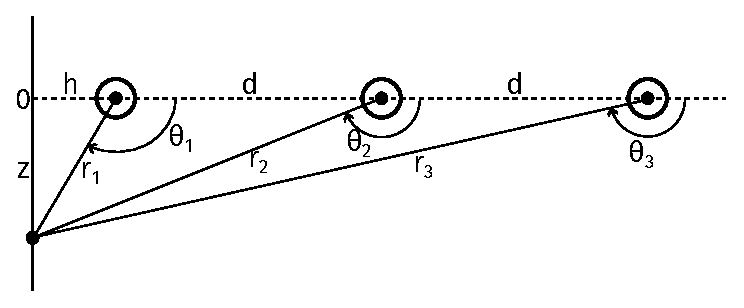
\includegraphics[width=0.45\textwidth]{../figures/horizontal_rms.eps}
%   \caption{RMS electric field magnitude, horizontal configuration.}
%   \label{fig:horizontal_rms}
% \end{figure}
% %
% Recalling that $r_\alpha = \nicefrac{\xi}{e_\alpha}$, we restrict the motion on
% the vertical line to obtain the constraints 
% \begin{align*}
%     -\frac{\xi}{e_\alpha}c_\alpha &= h
% + (\alpha - 1)d \;\; \Rightarrow \;\; e_\alpha = -\frac{\xi
% c_\alpha}{h+(\alpha-1)d}, \\
% \tan{\theta_\alpha} &=
% \frac{h+(\alpha-1)d}{z}, \qquad \alpha = 1, 2, 3.
% \end{align*}
% Plugging these relations into equation~\eqref{eq:rms} we find
% \[
% \bar{E}^2 = \frac{d^2 \xi ^2 \left(3 h^2+6 h d+4 d^2+3 z^2\right)}{2
% \left(h^2+z^2\right) \left((h+d)^2+z^2\right) \left((h+2 d)^2+z^2\right)}.
% \]
% %
% Taking the derivative of this expression with respect to $z$ and setting equal
% to zero, we find that the only real extremum point of this function is located
% at $z=0$.
% 
% 
% \subsubsection{Vertical Configuration}
% %
% Consider the vertical configuration, depicted in Figure~\ref{fig:vertical_rms}.
% The sensor is again restricted to lie on the vertical line, $h$\,\SI{}{\meter}
% away in the horizontal direction from all sensors. For simplicity, we assume
% that the middle transmission line is located at an altitude of $z=0$. The
% sensor is found a vertical distance $z$ away.
% %
% \begin{figure}[bt]
%   \centering
%   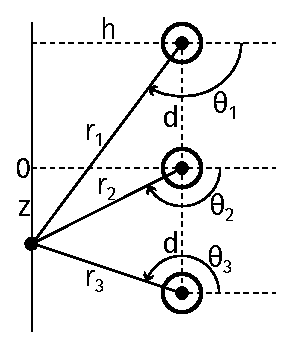
\includegraphics[width=0.175\textwidth]{../figures/vertical_rms.eps}
%   \caption{RMS electric field magnitude, vertical configuration.}
%   \label{fig:vertical_rms}
% \end{figure}
% %
% When the motion is restricted on this vertical line, the following constraints
% arise 
% %
% \begin{align*}
% \frac{\xi}{e_\alpha}\cos{\theta_\alpha} &= -h \;\; \Rightarrow \;\; e_\alpha =
% -\frac{\xi}{h}c_\alpha, \\
% \tan{\theta_\alpha} &= \frac{z+(2-\alpha)d}{h}, \quad \alpha = 1, 2, 3.
% \end{align*}
% %
% Plugging these relationships into equation~\eqref{eq:rms}, we find
% \[
% \bar{E}^2 = \frac{d^2 \xi ^2 \left(3 h^2+d^2+3 z^2\right)}{2
% \left(h^2+z^2\right) \left(h^2+(d-z)^2\right) \left(h^2+(d+z)^2\right)}
% \]
% %
% Taking the derivative of this expression with respect to $z$ and setting equal
% to zero, we find that if $h > \frac{884434}{1.6 \times 10^6}d$, the only real
% extremum point of this function is located at $z=0$.
% 
% 
% \subsubsection{Isosceles Triangle Configuration}
% %
% Consider the isosceles triangle configuration, depicted in
% Figure~\ref{fig:isosceles_rms}. The sensor is restricted to lie on the vertical
% line, $h$\,\SI{}{\meter} and $h^\prime$\,\SI{}{\meter} away from top/bottom and
% middle wires, respectively. We still assume that he middle transmission line is
% located at an altitude of $z=0$ and the sensor is found a vertical distance $z$
% away.
% %
% \begin{figure}[b]
%   \centering
%   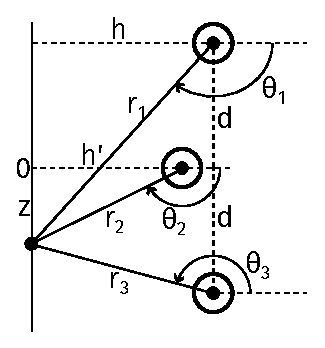
\includegraphics[width=0.2\textwidth]{../figures/isosceles_rms.eps}
%   \caption{RMS electric field magnitude, isosceles configuration.}
%   \label{fig:isosceles_rms}
% \end{figure}
% %
% When the motion is restricted on this vertical line, the following constraints
% arise 
% %
% \begin{align*}
%     e_1 &= -\frac{\xi}{h}c_1, \;\; e_2 = -\frac{\xi}{h^\prime}c_2, \;\; e_3 =
%     -\frac{\xi}{h}c_3,  \\
%     \tan{\theta_1} &= \frac{z+d}{h}, \;\; \tan{\theta_2} = \frac{z}{h^\prime},
%     \;\;
%     \tan{\theta_3} = \frac{z-d}{h}.
% \end{align*}
% %
% Plugging these relationships into equation~\eqref{eq:rms}, we find $\bar{E}^2 =
% \frac{p(z)}{q(z)}$, where 
% %
% \begin{align*}
%     p(z) &= \xi ^2 \left(d^4+d^2 \left(2 h^2-2 h h^\prime+3
% \left({h^\prime}^2+z^2\right)\right)+\right. \\
%          &\phantom{1234}\left. (h-h^\prime)^2 \left(h^2+z^2\right)\right), \\
%     q(z) &= 2 \left({h^\prime}^2+z^2\right)
% \left((d-z)^2+h^2\right) \left((d+z)^2+h^2\right).
% \end{align*}
% %
% Taking the derivative of this expression with respect to $z$ and setting equal
% to zero, we find that under many typical conditions, the only real extremum
% point of this function is located at $z=0$. For example, if $h^\prime = h -
% \delta$, then we only require that $d > \delta(-1 + \sqrt{2})$ for $z=0$ to be
% the unique extremum of $\bar{E}$.
% 
% 
% 
% \subsubsection{Crooked Configuration}
% 
\subsection{Control using Estimation}
\label{ssec:ctrl_w_est}

In Section~\ref{sec:estimation}, we have derived a method to localize a drone
with respect to a three-phase transmission line. A drone that is capable of
obtaining measurements of the electric and magnetic field around a three-phase
transmission line can leverage these signals to control its pose so that it can
install or retrieve a sensor package.

Suppose that the drone wants to approach a power line along its body
$\bm{x}$-axis in order to successfully snap-install a sensor package on it. For
such a manipulation, we desire that the drone's body $\bm{y}$-axis be aligned
axially with the power line and the drone's body $\bm{z}$-axis be aligned with
the gravity vector. We will assume that the drone's orientation is controlled
such that its $\bm{z}$-axis is always aligned with the gravity vector.

Since the power flows along axially along the wire, the Poynting
vector~\cite{griffiths2014introduction}, given by $\bm{P} = \bm{E} \times
\bm{H}$ points axially along the wire and its direction may be computed in the
body-frame of the drone through the sensor measurements of $\bm{E}$ and
$\bm{B}$. This reports the Poynting vector $\bm{P}$ in the body-coordinates as
well. We then form the cost function \[ \mc{J} = 1 - \hat{\bm{P}} \cdot
\hat{\bm{y}} = 1 -  \hat{p}_y, \] where $\hat{\bm{P}}$ is the unit vector along the
Poynting vector and $\hat{\bm{y}}$ is the unit vector along the body
$\bm{y}$-axis of the drone.

This cost function $\mc{J}$ is a function of the yaw angle $\psi$ of the drone.
Hence we can connect a spring to the minimizer of this cost function by
introducing a control term that flows along the negative gradient of $\mc{J}$
with respect to the angle between $\hat{\bm{P}}$ and $\hat{\bm{y}}$. \[\tau_z
= -k\hat{p}_x + \tau_d, \] where $\tau_d$ is a damping term that asymptotically
stabilizes angle such that the drone's $\bm{y}$-axis aligns with the axis of the
power line.

Once the body $\bm{y}$-axis of the drone is aligned with the long axis of the
power line, the translation of the drone may be controlled such that the
$\bm{z}$-component, $E_z$ of the electric field vanishes. This is accomplished
by gaining altitude such that the altitude of the drone matches that of the
power line. The reference altitude to achieve is provided by the bearing angle,
without loss of generality, assumed to be $\theta_1$ from
Section~\ref{sec:estimation}. Depending on which side of the power line the
drone is we want to control $\theta_1$ such that either $\theta_1 \rightarrow 0$
or $\theta_1 \rightarrow \pi$. In either case, the angle $\theta_1$ is given as
a function of the $(x, z)$ location of the drone by \[\theta_1 = \arctan{\left(
\frac{z_1 - z}{x_1-x} \right)}, \] where $(x, z)$ and $(x_1, z_1)$ are the
locations of the drone and the wire with respect to the world frame. If we want
to drive $E_z \rightarrow 0$, then we can take as cost function $\mc{J} = 1 -
\cos{\theta_1}$ if we want $\theta_1 \rightarrow 0$ or $\mc{J} =
1+\cos{\theta_1}$ if we want $\theta_1 \rightarrow \pi$. For example, in case
$\theta_1 \rightarrow 0$ is desired, taking the gradient of the corresponding
function with respect to $z$ we obtain \[ \pd{\mc{J}}{z} =
\frac{\sin{\theta_1}\cos{\theta_1}}{r_1}, \] where $r_1$ is the radial distance
to the transmission wire. Since each of these quantities are estimated in the
procedure outlined in Section~\ref{sec:estimation}, we can instruct the drone to
move by the negative of this amount in the body $\bm{z}$-direction, which will
achieve $\theta_1 \rightarrow 0$. Once the desired value for $\theta_1$ is
achieved, a controlled body $\bm{x}$-axis motion is all that is needed to
install a sensor on the power line of interest.

% Let us denote the yaw angle of the drone, acting along its body $\bm{z}$-axis by
% $\psi$. We construct a desired value $\psi_d$ for the yaw angle 
% In order to align the drone's body $\bm{y}$-axis axially along the wire,
